\documentclass[10pt,a4paper,titlepage]{report}
\usepackage[utf8]{inputenc}
\usepackage{amsmath}
\usepackage{amsfonts}
\usepackage{amssymb}
\usepackage{graphicx}
\usepackage{xcolor}
\usepackage{minted}

\newcommand{\HRule}[1]{\rule{\linewidth}{#1}}

\nonstopmode


\begin{document}
{\fontfamily{cmr}\selectfont
\title{ \normalsize \textsc{}
\\ [2.0cm]
\HRule{0.5pt} \\
\LARGE \textbf{\uppercase{basic sql queries i}
\HRule{2pt} \\ [0.5cm]
\normalsize \today \vspace*{5\baselineskip}}
}

\date{}

\author{
	Rwithik Manoj \\
	College of Engineering, Trivandrum \\
	Department of Computer Science and Engineering }

\maketitle
\newpage

\sectionfont{\scshape}

\begin{enumerate}
		\item Display the details of all the employees.\newline
			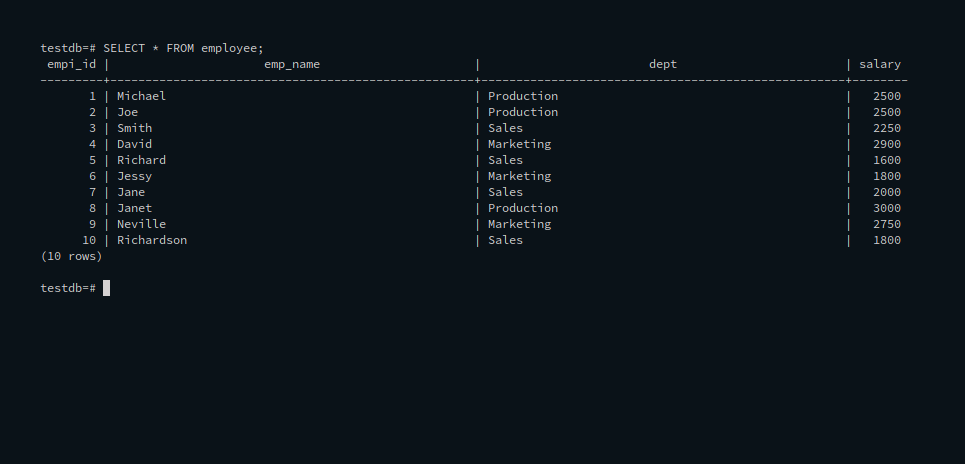
\includegraphics[width=\linewidth]{../Images/Basics/1.png}\newline
		\item Display the names and id’s of all employees.\newline
			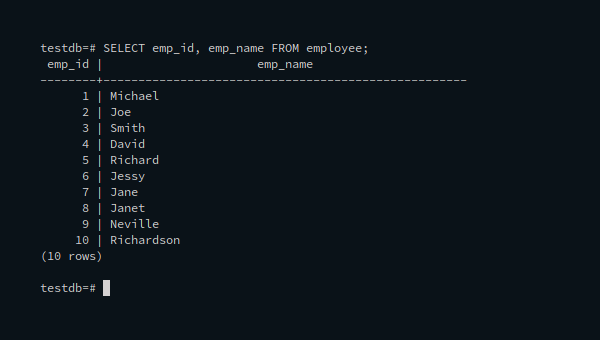
\includegraphics[width=\linewidth]{../Images/Basics/2.png}\newline
		\item Delete the entry corresponding to employee id:10.\newline
			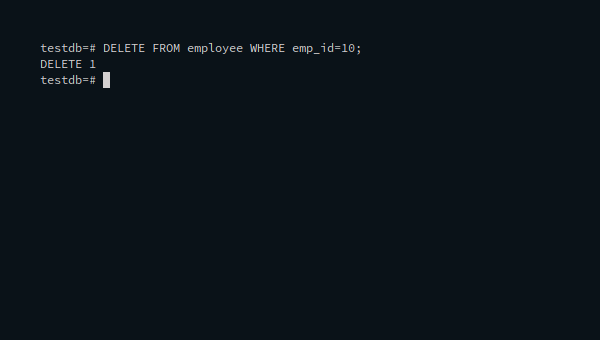
\includegraphics[width=\linewidth]{../Images/Basics/3.png}\newline
		\item Insert a new tuple to the table. The salary field of the new employee should be kept NULL.\newline
			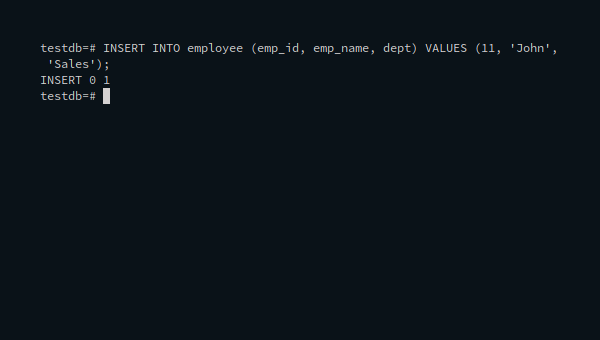
\includegraphics[width=\linewidth]{../Images/Basics/4.png}\newline
		\item Find the details of all employees working in the marketing department.\newline
			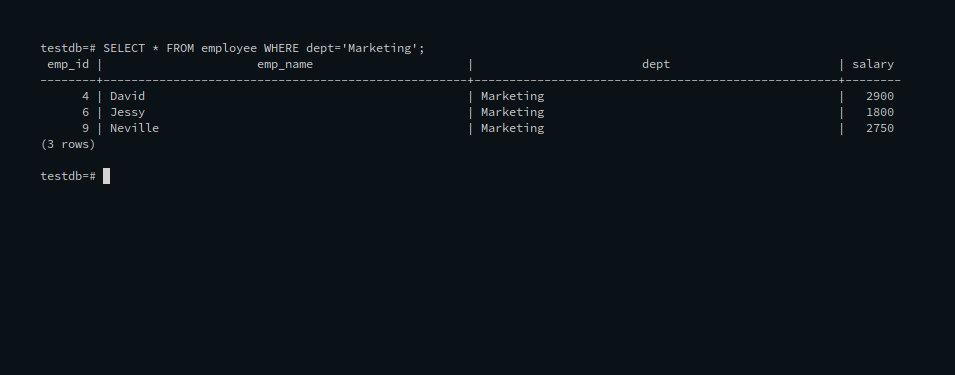
\includegraphics[width=\linewidth]{../Images/Basics/5.png}\newline
		\item Add the salary details of the newly added employee.\newline
			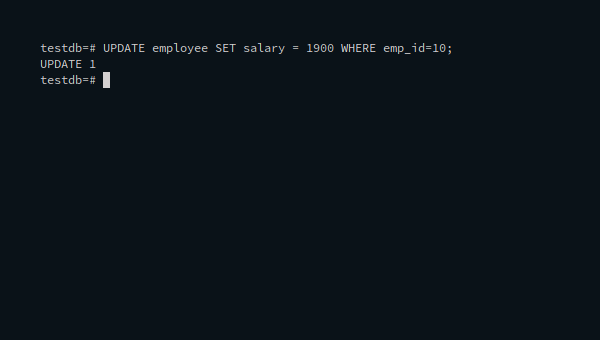
\includegraphics[width=\linewidth]{../Images/Basics/6.png}\newline
		\item Update the salary of Richard to 1900\$.\newline
			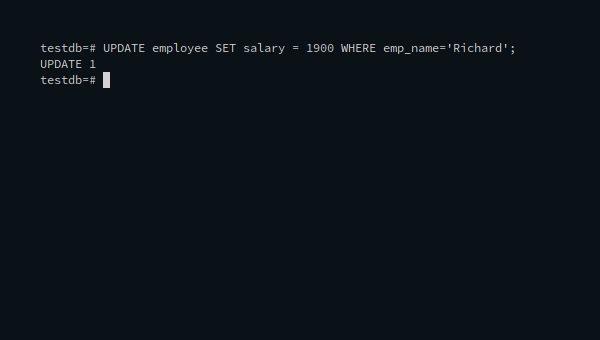
\includegraphics[width=\linewidth]{../Images/Basics/7.png}\newline
		\item Find the details of all employees who are working for marketing and has a salary greater than	2000\$.\newline
			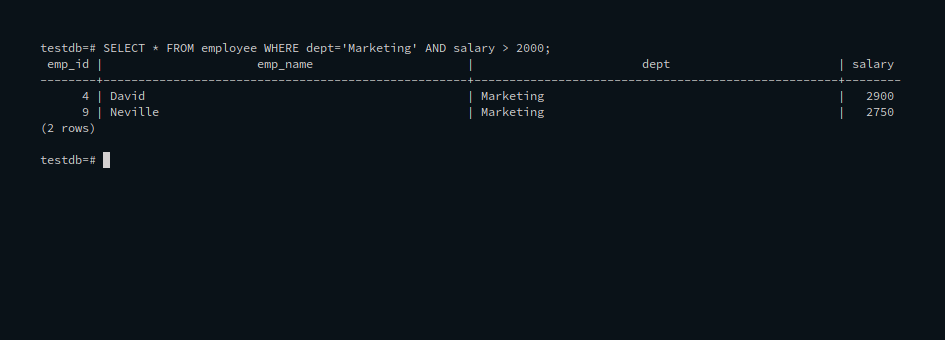
\includegraphics[width=\linewidth]{../Images/Basics/8.png}\newline
		\item List the names of all employees working in the sales department and marketing department.\newline
			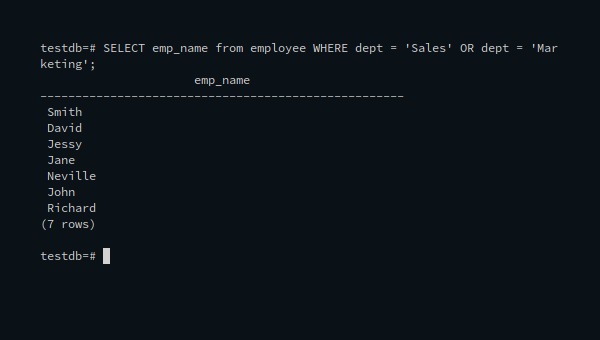
\includegraphics[width=\linewidth]{../Images/Basics/9.png}\newline
		\item List the names and department of all employees whose salary is between2300\$ and 3000\$.\newline
			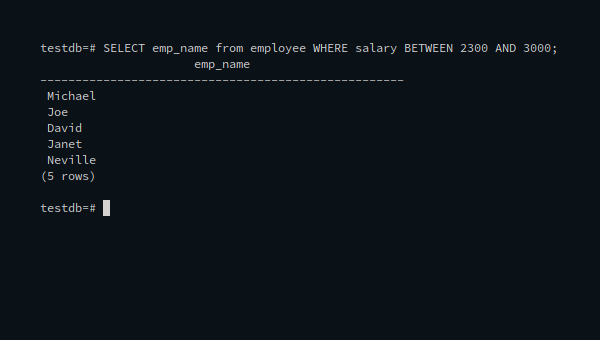
\includegraphics[width=\linewidth]{../Images/Basics/10.png}\newline
		\item Update the salary of all employees working in production department 12\%.\newline
			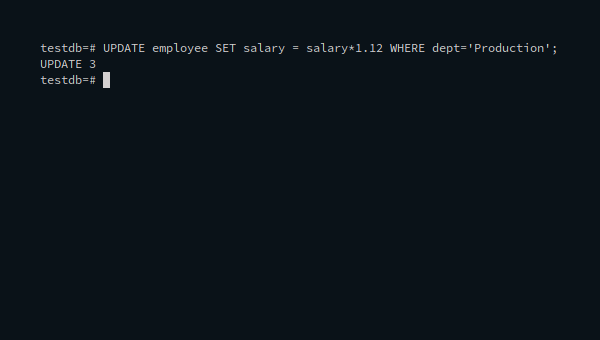
\includegraphics[width=\linewidth]{../Images/Basics/11.png}\newline
		\item Display the names of all employees whose salary is less than 2000\$ or working for sales department.\newline
			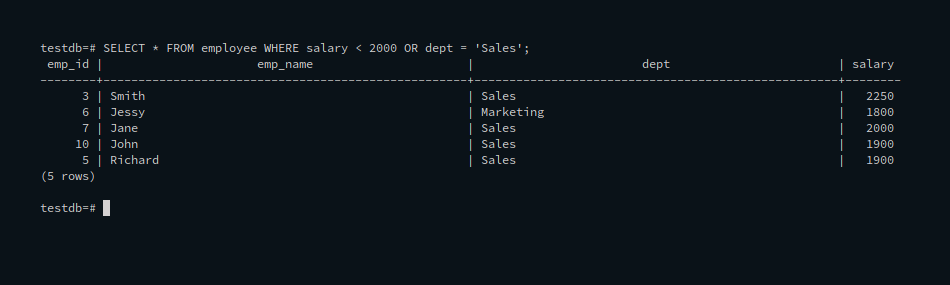
\includegraphics[width=\linewidth]{../Images/Basics/12.png}\newline
\end{enumerate}

\subsubsection*{RESULT}

The query was executed and the output was obtained.


}
\end{document}
